\section{Construction of the ODE Model}
\label{sec:wo_detect}
We investigate the selfish detection in this and the following sections.
Specifically, in this section, the ordinary differential equation model
is constructed to capture the state change with time.
\subsection{Without Detection}
\begin{figure}
  \centering
  {\includegraphics[width=0.25\textwidth]
  {fig/state_transition_no_detect.eps}}
     \caption{State transition of the relay nodes without detection.}
     \label{fig:ss_wo_dt}
\end{figure}
First, we analyze the change of the network state with time
when the selfish detection is not deployed. 
The state transition is shown
in Fig.~\ref{fig:ss_wo_dt} with the following rules.
The nodes change from state $R$ to state $I$ if they contact $src$.
The corresponding incremental rate of state $I$ is $\lambda R(t)$ at time $t$. 
The selfish node also may contact $src$ in the opportunistic network.
Then the total incremental rate of $I$ is 
$\lambda (R(t)+D(t))=\lambda (N-I(t))$.
Additionally, the infected node may become the selfish node with rate $\rho$.
Thus we can obtain the derivative of $I(t)$ with respect to $t$,
\begin{small}
\begin{equation}
\nonumber
\begin{aligned}
\frac{\mathrm{d} I(t)}{\mathrm{d} t} &= \lambda (N-I(t)) - \rho I(t).
\end{aligned}
\end{equation}
\end{small}
where $\lambda$ and $\rho$ are constants.
Similar to $\frac{\mathrm{d} I(t)}{\mathrm{d} t}$,
we can get the change rate of state $D$ and state $R$,
i.e. $\frac{\mathrm{d} D(t)}{\mathrm{d} t}$ and
$\frac{\mathrm{d} R(t)}{\mathrm{d} t}$,
and obtain the model,
\begin{small}
\begin{equation}
\label{eq:IDR_wo}
\begin{aligned}
\frac{\mathrm{d} I(t)}{\mathrm{d} t} &=  \lambda (N-I(t)) - \rho I(t),\\
\frac{\mathrm{d} D(t)}{\mathrm{d} t} &= - \lambda D(t) + \rho I(t),\\
\frac{\mathrm{d} R(t)}{\mathrm{d} t} &= - \lambda (N-I(t)-D(t)),
\end{aligned}
\end{equation}
\end{small}
Since (\ref{eq:IDR_wo}) is formed by the first-order first-power
ordinary differential equations,
we can calculate the general solutions of it, that is,
\begin{small}
\begin{equation}
\nonumber
\begin{aligned}
I(t) = C e^{-(\lambda + \rho)t} + \frac{ \lambda N }{ \lambda + \rho }.
\end{aligned}
\end{equation}
\end{small}

At first, $M(0)=0$ and $I(0)=0$, only $src$ has the messages.
Note that $0 \le I(t) \le N$ and $0 \le M(t) \le N$.
We use $\dot{I}$ and $\dot{M}$ denote $I(t)$ and $M(t)$.
Following the two-hop routing,
where only the source node can replicate the message to other nodes,
we get that the corresponding ODEs like~\cite{CC2007PerfAnaly}, which are

when $0 \le I(t) \le N$ and $0 \le M(t) \le N$.

And then we find the close-form value of $I(t)$ and $M(t)$ to ensure $I_{s}$ and $M_{s}$.
From the first ODE, $\dot{I} + \rho I = \beta (N-I)$, we can obtain

Considering that $I(t=0) = 0$, $C = \frac{ -\beta N }{ \beta + \rho }$.
Thus
\begin{small}
\begin{equation}
\nonumber
\begin{aligned}
I(t) = \frac{ \beta N }{ \beta + \rho } - \frac{ \beta N }{ \beta + \rho } e^{-(\beta + \rho)t}.
\end{aligned}
\end{equation}
\end{small}

Similarly, from $\dot{M} + \beta M = \rho I$,
\begin{small}
\begin{equation}
\nonumber
\begin{aligned}
M(t) &= C e^{-\int \beta dt} + e^{-\int \beta dt} \int \rho I e^{\int \beta dt} dt \\
&= C e^{- \beta t} + e^{- \beta t} \int \rho \frac{ \beta N }{ \beta + \rho } (1 - e^{-(\beta + \rho)t}) e^{ \beta t} dt \\
&= C e^{- \beta t} + \frac{ \beta N }{ \beta + \rho } e^{-(\beta + \rho)t} + \frac{ \rho N }{ \beta + \rho }
\end{aligned}
\end{equation}
\end{small}
Because of $M(0)=0$,
\begin{small}
\begin{equation}
\nonumber
\begin{aligned}
M(t) &= -N e^{- \beta t} + \frac{ \beta N }{ \beta + \rho } e^{-(\beta + \rho)t} + \frac{ \rho N }{ \beta + \rho }
\end{aligned}
\end{equation}
\end{small}
\begin{figure}
  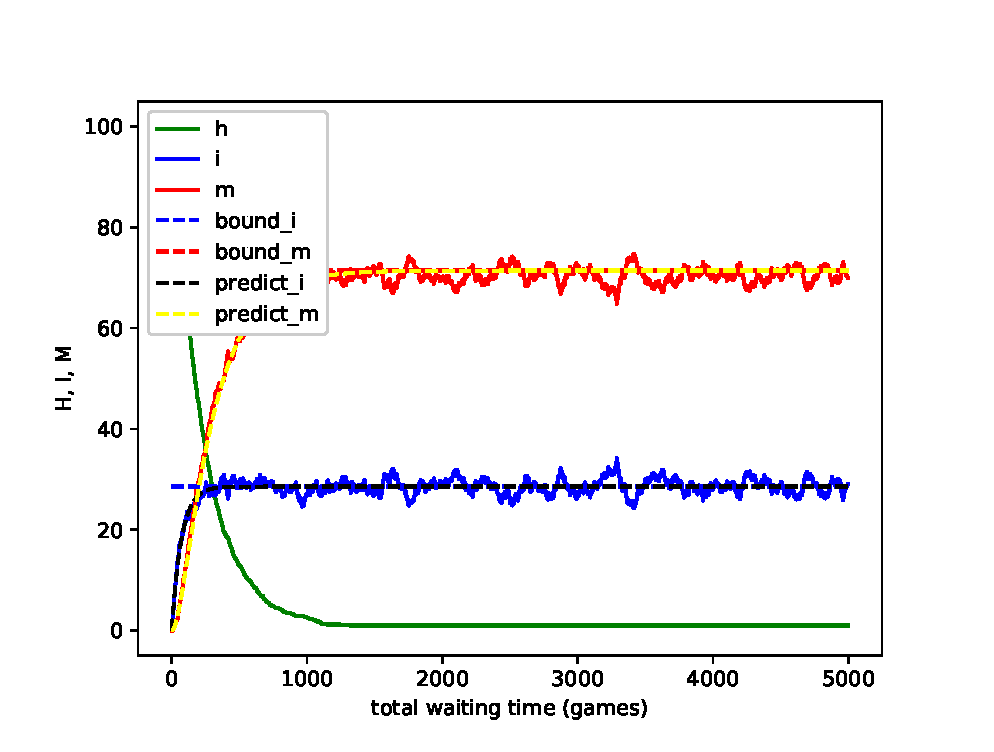
\includegraphics[width=.45\textwidth]{fig/twohop_predict_sim.eps}
  \caption{$I(t)$ and $M(t)$ with time $t$ obtained from prediction and simulations
  when $\beta = 0.004$, $\rho = 0.01$ and $N=100$. Here $h$ and $i$ is the mean value of $20$ simulations.}
  \label{fig:twohop_predict_wod}
\end{figure}
We can find that when $t \rightarrow + \infty$, $I(t) \rightarrow \frac{ \beta N }{ \beta + \rho }$
and $M(t) \rightarrow \frac{ \rho N }{ \beta + \rho }$.

\subsection{Object Function}
The expected number of nodes, which declare that holding the messages, in the range $t \in (0, T]$
can be viewed as the contribution of the relay nodes,
which will be proportional to the reward paid from the message sender.
Thus the total paid reward for the selfish behaviors is
\begin{small}
\begin{equation}
\nonumber
\begin{aligned}
J &= \int_{0}^{T} M(t) dt,
\end{aligned}
\end{equation}
\end{small}
where $T$ is the Time to Live (TTL) of message $m$.
$M(t)$ is the waste of the reward at the instant time $t$.
which also can be calculated.
Based on the calculated result,
We can find that $()\%$ reward are paid to the nodes without messages.

